\documentclass[a6paper, 10pt, twoside]{article}
%\usepackage[T1]{fontenc}
\usepackage[british]{babel}
\usepackage[utf8]{inputenc}
\usepackage{float, graphicx,amsmath,amsfonts,cite,enumerate,tabularx}
\usepackage[final]{pdfpages}
\usepackage{wrapfig}
\usepackage[margin=0.3in]{geometry}
\usepackage{sidspaltHack}
\usepackage{digital}

\setlength{\oddsidemargin}{-0.37in}
\setlength{\evensidemargin}{-0.47in}
\setlength{\textwidth}{215pt}

\pagestyle{empty}

\begin{document}
\nysida{10}{1}
\noindent
\chaptertitlenobr{K$\kappa$}{Fina visor}
\small
\begin{center}
\songtitle{$\kappa1$}{Festen skall börjas} 
\mel{Vårvindar friska}
\end{center}
\begin{lyrics}
Festen skall börjas, kråset ska smörjas\\
magen skall få det som den vill ha.\\
Glasen står fulla, låt sången rulla.\\
Glädjen skall vara gäst här i da.
\vspace{5pt}\\
Glasen i handen fatta och sjung\\
glöm alla sorger, var bara ung.\\
Glöm morgondagen.\\
Tänk blott på magen.\\
Skål alla vänner! Hej och gutår!
\end{lyrics}
\vfill
\begin{figure}[!h]
\centering

\includegraphics[width=1.0\textwidth]{fin.jpg}
\end{figure}

\nysida{10}{2}
\noindent
\begin{center}
\songtitle{$\kappa2$}{Festvisa} 
\mel{Sjösala vals}
\end{center}
\begin{lyrics}
Årets första fest sker på klassiskt manér,\\
känn hur glädjen spritter uti kroppen med väldig fart.\\
Börja lätt med ölen ty den går alltid ner,\\
å innan festens slut sänkes nog några fler.
\vspace{5pt}\\
Smaka nu på bäsken, det ädla fabrikat,\\
om kryddan bränner strupen finns bättre destillat.\\
Ty punschen kommer ljuv och sval,\\
läskar ända in i märgen.\\
Nu ska vi roa oss kungligt till klockan fem.
\end{lyrics}
\auth{n$\emptyset$llespexet 2004}
\begin{center}
\songtitle{$\kappa3$}{Sjösala vals} 
\end{center}
\begin{lyrics}
Rönnerdahl han skuttar med ett skratt ur sin säng.\\
Solen står på Orrberget. Sunnanvind brusar.\\
Rönnerdahl han valsar över Sjösala äng.\\
- Hör min vackra visa, kom sjung min refräng!
\vspace{5pt}\\
Tärnan har fått ungar och dyker i min vik,\\
ur alla gröna dungar hörs finkarnas musik,\\
och se, så många blommor som redan \\
slagit ut på ängen!\\
Gullviva, mandelblom, kattfot och blå viol.
\vspace{5pt}\\
Rönnerdahl han virvlar sina lurviga ben,\\
under vita skjortan som viftar kring vadorna.\\
Lycklig som en lärka uti majsolens sken,\\
sjunger han för ekorr'n, som gungar på gren!
\nysida{10}{3}
\noindent
- Kurre, kurre, kurre! Nu dansar Rönnerdahl!\\
Koko! Och göken ropar uti hans gröna dal\\
och se, så många blommor som redan \\
slagit ut på ängen!\\
Gullviva, mandelblom, kattfot och blå viol.
\vspace{5pt}\\
Rönnerdahl han binder utav blommor en krans,\\
binder den kring håret, det gråa och rufsiga,\\
valsar in i stugan och har lutan till hands,\\
väcker frun och barnen med drill och kadans.
\vspace{5pt}\\
- Titta ropar ungarna, Pappa är en brud\\
med blomsterkrans i håret och nattskjorta till skrud!\\
Och se, så många blommor som redan \\
slagit ut på ängen!\\
Gullviva, mandelblom, kattfot och blå viol.
\vspace{5pt}\\
Rönnerdahl är gammal, men han valsar ändå!\\
Rönnerdahl har sorger och ont om sekiner.\\
Sällan får han rasta - han får slita för två.\\
Hur han klarar skivan, kan ingen förstå
\vspace{5pt}\\
Ingen utom tärnan i viken, hon som dök\\
och ekorren och finken och vårens första gök\\
och blommorna, de blommor som redan \\
slagit ut på ängen!\\
Gullviva, mandelblom, kattfot och blå viol. 
\end{lyrics}
\auth{Evert Taube}
% TODO: There is a bug where if \nysida is called within the lyrics environment, it stops having an effect after \end{lyrics}
% Hence we need to renew the sidspaltindex here.
\sidindex{10}{3}

\nysida{10}{4}
\noindent
\begin{center}
\songtitle{$\kappa4$}{Änglamark} 
\end{center}
\begin{lyrics}
Kalla den änglamarken eller himlajorden om du vill,\\
jorden vi ärvde och lunden den gröna.\\
Vildrosor och blåklockor \physicalonly{\\}och lindblommor och kamomill.\\
Låt dem få leva, de är ju så sköna.
\vspace{5pt}\\
Låt barnen dansa som änglar kring lönn och alm,\\
leka tittut mellan blommande grenar.\\
Låt fåglar flyga och sjunga för oss sin psalm.\\
Låt fiskar simma bland bryggor och stenar.
\vspace{5pt}\\
Sluta att utrota skogarnas alla djur!\\
Låt örnen flyga, låt rådjuren löpa!\\
Låt sista älven som brusar i vår natur\\
brusa alltjämt mellan fjällar och gran och fur!
\vspace{5pt}\\
Kalla den änglamarken eller himlajorden om du vill,\\
jorden vi ärvde och lunden den gröna.\\
Vildrosor och blåklockor \physicalonly{\\}och lindblommor och kamomill.\\
Låt dem få leva, de är ju så sköna.
\end{lyrics}
\auth{Evert Taube}
\begin{figure}[!h]
\centering
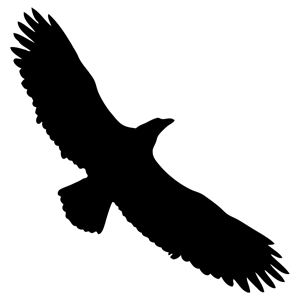
\includegraphics[width=0.4\textwidth]{eagle.png}
\end{figure}

\nysida{10}{5}
\noindent
\begin{center}
\songtitle{$\kappa5$}{Fritiof och Carmencita} 
\end{center}
\begin{lyrics}
Samborombon, en liten by förutan gata, \\
den ligger inte långt från Rio de la Plata. \\
Nästan i kanten av den blåa Atlanten \\
och med Pampas bakom sig \\
många hundra gröna mil. \\
Dit kom jag ridande en afton i april, \\
för jag ville dansa tango. 
\vspace{5pt}\\
Dragspel, fiol och mandolin \\
hördes från krogen och i salen steg jag in. \\
Där på bänken i mantilj \\
och med en ros vid sin barm\\
satt den bedårande lilla Carmencita. \\
Mamman, värdinnan satt i vrån, \\
hon tog mitt ridspö, min pistol och min manton. \\
Jag bjöd upp och Carmencita sa: \\
'Si gracias señor. Vamos á bailár este tango.' 
\vspace{5pt}\\
Carmencita lilla vän, håller du utav mig än? \\
Får jag tala med din pappa och din mamma, \\
jag vill gifta mig med dig, Carmencita! \\
Nej, don Fritiof Andersson, kom ej till Samborombon \\
om ni hyser andra planer när det gäller mig, \\
än att dansa tango. 
\vspace{5pt}\\
Ack, Carmencita gör mig inte så besviken, \\
jag tänker skaffa mig ett jobb här i butiken, \\
sköta mig noga, bara spara och knoga \\
inte spela och dricka, men bara älska dig. \\
Säg, Carmencita, det är ändå blott med mig, \\
säg, som du vill dansa tango. 

\newpage
\noindent
Nej Fritiof, ni förstår musik, \\
men jag tror inte ni kan stå i en butik \\
och förresten sa min pappa just idag att han visste, \\
vem som snart skulle fria till hans dotter. \\
En som har tjugotusen kor, \\
och en estancia som är förfärligt stor. \\
Han har prisbelönta tjurar, \\
han har oxar, kor och svin \\
och han dansar underbar tango. 
\vspace{5pt}\\
Carmencita, lilla vän, akta dig för rika män! \\
Lyckan den bor ej i oxar eller kor \\
och den kan heller inte köpas för pengar. \\
Men min kärlek gör dig rik, \\
skaffa mig ett jobb i er butik. \\
Och när vi blir gifta söta ungar skall vi få, \\
som kan dansa tango.
\end{lyrics}
\auth{Evert Taube}
	    
\nysida{10}{6}
\noindent
\begin{center}
\songtitle{$\kappa6$}{Än en gång däran} 
\end{center}
\begin{lyrics}
Än en gång däran, bröder,\\
än en gång däran,\\
följom den urgamla seden.\\
In till sista man, bröder,\\
in till sista man,\\
trotsa vi hatet och vreden. \\\digitalonly{\\}
Blankare vapen sågs aldrig i en här\\
än dessa glasen, kamrater i gevär!\\
Än en gång däran, bröder,\\
än en gång däran.\\
Svenska hjärtans djup - här är din sup!
\vspace{5pt}\\
Livet är så kort, systrar,\\
livet är så kort,\\
lek det ej bort, nej var redo!\\
Kämpa mot allt torrt, systrar,\\
kämpa mot allt torrt.\\
Tänk på de gamla som skredo\\\digitalonly{\\}
fram utan tvekan i floder av champagne.\\
Stärkta från början av brännvin från vårt land.\\
Kämpa mot allt torrt, systrar,\\
kämpa mot allt torrt.\\
Svenska hjärtans djup - här är din sup! 
\end{lyrics}
\auth{Evert Taube}

\nysida{10}{7}
\noindent
\begin{center}
\songtitle{$\kappa7$}{En liten blå förgätmigej}
% TODO: Digitalize
\small{\textit{Sjungs knästående för serveringspersonalen}}
\end{center}
\begin{lyrics}
Hur gärna ville jag ej vara,\\
en liten blå förgätmigej,\\
en liten blå förgätmigej.\\
Då skulle jag för dig förklara\\
hur innerligt jag älskar dig!
\end{lyrics}
\vspace{30pt}
\begin{center}
\songtitle{$\kappa8$}{Längtan till landet} 
\sheetmusicnotice{Noter till blandad kör finns i notkapitlet}
\end{center}
\begin{lyrics}
Vintern rasat ut bland våra fjällar,\\
drivans blommor smälta ned och dö.\\
Himlen ler i vårens ljusa kvällar,\\
solen kysser liv i skog och sjö.
\vspace{5pt}\\
$\|$: Snart är sommarn här i purpurvågor,\\
guldbelagda, azurskiftande,\\
ligga ängarne i dagens lågor,\\
och i lunden dansa källorne :$\|$
\vspace{5pt}\\
Ja, jag kommer! Hälsen glada vindar,\\
ut till landet, ut till fåglarne,\\
att jag älskar dem, till björk och lindar,\\
sjö och berg jag vill dem återse.
\vspace{5pt}\\
$\|$: Se dem än som i min barndoms stunder,\\
följa bäckens dans till klarnad sjö,\\
trastens sång i furuskogens lunder,\\
vattenfågelns lek kring fjärd och ö. :$\|$
\end{lyrics}
\auth{H. Sätherberg}

\nysida{10}{9}
\noindent
\begin{center}
\songtitle{$\kappa9$}{Balladen om Herr Fredrik Åkare och den söta fröken Cecilia Lind} 
\mel{Monday morning}
\end{center}
\begin{lyrics}
Från Öckerö loge hörs dragspel och bas\\
och fullmånen lyser som var den av glas.\\
Där dansar Fredrik Åkare kind emot kind\\
med lilla fröken Cecilia Lind.
\vspace{5pt}\\
Hon dansar och blundar så nära intill,\\
hon följer i dansen precis vart han vill.\\
Han för och hon följer så lätt som en vind,\\
Men säg varför rodnar Cecilia Lind?
\vspace{5pt}\\
Säg var det för det Fredrik Åkare sa:\\
Du doftar så gott och du dansar så bra.\\
Din midja är smal och barmen är trind.\\
Vad du är vacker, Cecilia Lind.
\vspace{5pt}\\
Men dansen tog slut och vart skulle dom gå?\\
Dom bodde så nära varandra ändå.\\
Till slut kom dom fram till Cecilias grind.\\
Nu vill jag bli kysst, sa Cecilia Lind.
\vspace{5pt}\\
Vet hut, Fredrik Åkare, skäms gamla karln!\\
Cecilia Lind är ju bara ett barn.\\
Ren som en blomma, skygg som en hind.\\
Jag fyller snart sjutton, sa Cecilia Lind.
\vspace{5pt}\\
Och stjärnorna vandra och timmarna fly\\
och Fredrik är gammal men månen är ny.\\
Ja, Fredrik är gammal men kärlek är blind.\\
Åh, kyss mig igen, sa Cecilia Lind.
\end{lyrics}
\auth{Text: Cornelis Vreeswijk}

\nysida{10}{10}
\noindent
\begin{center}
\songtitle{$\kappa10$}{Hårgalåten} 
\end{center}
\begin{lyrics}
Spelaren drog fiol'n ur lådan och\\
lyfte stråken högt mot söndagsolens kula.\\
Då blev det fart i Hårgafolket,\\
de glömde Gud och hela världen.
\vspace{5pt}\\
Dansen gick på äng och backar\\
högt upp på Hårgaåsens topp.\\
De slet ut båd skor och klackar,\\
aldrig fick en på dansen stopp.
\vspace{5pt}\\
Varifrån kommer du som spelar\\
säg vem har lärt dig detta spel, det vilda, det galna.\\
Stannar du inte brister hjärtat;\\
O Gud bevare, hen har bockfot!
\vspace{5pt}\\
Klockorna hade ringt i dalen och där gick\\
far och mor och bror till sockenkyrkan.\\
Var kan nu Hårgas ungdom vara?\\
Å herregud de dansar ännu!
\vspace{5pt}\\
Dansen går till Hårgalåten\\
högt upp på Hårgaåsens topp.\\
De har inte långt till gråten,\\
dansar nu sönder själ och kropp.
\vspace{5pt}\\
Hejda din stråke spelare innan \\
vi dansar liv och själ och alla ben ur kroppen.\\
Nej inte slutar hen sin dans \\
förr'n de allesammans faller döda.
\end{lyrics}

\nysida{10}{11}
\noindent
\begin{center}
\songtitle{$\kappa11$}{En dansk aquavit} 
\end{center}
\begin{lyrics}
Ren som en jomfru\\
og stærk som en bejler,\\
hed som det hjærte,\\
der hamre mod dit.
\vspace{5pt}\\
Kølig som kilden,\\
der vårhimlen spejler:\\
$\|$: sådan min ven,\\
er en dansk aquavit. :$\|$ 
\end{lyrics}
\auth{Hans Hartvig Seedorf}
\begin{center}
\songtitle{$\kappa12$}{Trink, trink} 
\end{center}
\begin{lyrics}
Trink, trink, Brüderlein\digitalonly{/Schwesterlein} trink\\
Lasset die Sorgen zu Haus\\
Trink, trink, Brüderlein\digitalonly{/Schwesterlein} trink\\
Bald ist das Leben aus
\vspace{5pt}\\
$\|$: Meide den Kummer und meide den Schmerz\\
Dann ist das Leben ein Schertz :$\|$
\vspace{5pt}\\
Trink... etc.
\vspace{5pt}\\
$\|$: Meide die Weiber und meide das Bier\\
Dann wird ein Sportsman aus dir :$\|$
\vspace{5pt}\\
Trink... etc.
\vspace{5pt}\\
$\|$: Heirat im Sommer und scheide in März\\
Dann ist das Leben ein Schertz :$\|$
\vspace{5pt}\\
Trink... etc.
\vspace{5pt}\\
$\|$: Kauf dir ein Auto, fahr gegen ein Baum\\
Dann wird das Leben ein Traum :$\|$
\end{lyrics}
\nysida{10}{13}
\noindent
\begin{center}
\songtitle{$\kappa13$a}{Smedsvisan\digitalonly{ (Smedsvisa från uppland)})}
\sheetmusicnotice{Noter finns i notkapitlet}
\end{center}
\begin{lyrics}
En gång i min ungdom älskade jag\\
en mänska med rena och sköna behag.\\
Hen lovfte mig tro, i lust och i nöd\\
allt in till sin blekaste död.
\vspace{5pt}\\
Hej hopp faderi faderalladerej!\\
Hej hopp faderi faderalladerej!\\
Hen lovfte mig tro, i lust och i nöd\\
allt in till sin blekaste död.
\vspace{5pt}\\
Hen var som en lilja vit uti hyn\\
den vackraste mänska en skådat i byn.\\
Ett smittande skratt, en lustiger sång\\
vi älskade sommaren lång.
\vspace{5pt}\\
Hej hopp faderi faderalladerej!\\
Hej hopp faderi faderalladerej!\\
Ett smittande skratt, en lustiger sång\\
vi älskade sommaren lång.
\vspace{5pt}\\
Men kärleken vissna', kärleken dog\\
vid Mikaels mässa den mänskan fått nog.\\
Hen fann sig en riker och högfärdig själ,\\
sa "Tack och adjö och farväl".
\vspace{5pt}\\
Hej hopp faderi faderalladerej!\\
Hej hopp faderi faderalladerej!\\
Hen fann sig en riker och högfärdig själ,\\
sa "Tack och adjö och farväl".
\vspace{5pt}\\
Nu står jag vid städet sliten och grå\\
och hammaren bultar och hjärtat likså.\\
Den mänskan hen kommer aldrig igen,\\
hen är hos sin nyfunne vän.

\newpage
\noindent
Hej hopp faderi faderalladerej!\\
Hej hopp faderi faderalladerej!\\
Den mänskan hen kommer aldrig igen,\\
men sången den trallar jag än. 
\end{lyrics}
\auth{Daniel Helldén}
%\vspace{40pt}
\begin{center}
\songtitle{$\kappa13$b}{Korta smedsvisan}
\end{center}
\begin{lyrics}
En gång i min ungdom älskade jag - \\
Sa tack och adjö och försvann!
\end{lyrics}
\vspace{20pt}
\begin{center}
\songtitle{$\kappa14$}{Balladen om ett kärlekspar}
\end{center}
\begin{lyrics}
Två studenter på teknis \\
satt i skolan hand i hand. \\
Som epsilon och delta, \\
beroende av varann. \\
Med gemensamma intressen, \\
som kvarkar och primtal. \\
Blev kärleken oändlig, \\
som en exponential. 
\vspace{5pt}\\
Likt den trigonometriska ettan, \\
var summan av dem ett. \\
Och som linjer i ett spektrum, \\
satt de alltid ganska tätt. \\
I vartenda koordinatsystem \\
var lyckan invariant. \\
Och beloppet av deras kärlek \\
var en enda stor konstant. \\
\nysida{10}{14}
\noindent
Kärlekens kurva, \\
en approximation \\
som långt bortom t0, \\
ger extrapolation. \\
De räknade tillsammans, \\
på varje fråga fanns ett svar. \\
Men i grund och botten var dem \\
ett kärlekspar.
\vspace{5pt}\\
De var summan ifrån ett till två, \\
som var upphöjd till nåt jämnt. \\
Likt en stillsam laserstråle, \\
var dialogen koherent. \\
Deras lycka var som värmebad \\
med en inre energi \\
som var svår att definiera, \\
såsom ordet exergi.
\vspace{5pt}\\
Men denna osäkerhetsrelation \\
var i klassisk obalans \\
Och ett gräl som var försumbart \\
fick oändlig resonans. \\
De såg från skilda vinklar, \\
från theta och från fi. \\
Vilket ledde till ett kaos, \\
och en ökad entropi.
\vspace{5pt}\\
Kärlekens kurva, \\
en approximation \\
som långt bortom t0, \\
blir superposition. \\
De var dolda variabler \\
och satt aldrig i en bar. \\
Men i andras ögon var de \\
ett kärlekspar. 
\newpage
\noindent
Deras lycka kom till toppen, \\
tangenten böjdes ner, \\
derivatan fick ett minus \\
och termerna blev fler \\
Snövit ifrån teknis \\
fick en kvadratrötterman \\
när likhetstecknet flydde \\
och förhållandet försvann.
\vspace{5pt}\\
Kärlekens kurva, \\
en taylorexpansion \\
som långt bortom t0, \\
ej har defintion. \\
Anonyma mänskor var de, \\
de var ordet som blev kvar. \\
Men tiden glömmer aldrig \\
detta kärlekspar.
\end{lyrics}
\auth{Tomi Ylinen, F-01}
% TODO: Sidindex-bugg, see TODO for Sjösala vals.
\sidindex{10}{14}

\nysida{10}{15}
\noindent
\begin{center}
\songtitle{$\kappa15$}{Stad i ljus}
\end{center}
\begin{lyrics}
Min resa var mot solen, \\
långt bortom alla slutna rum. \\
Där allting är oändligt, \\
och alla gränser har förevigt suddats ut.
\vspace{5pt} \\
Jag ville se miraklet, \\
och höra ord som föder liv. \\
Bli buren av en styrka, \\ 
som bara växer när jag anat mitt motiv. % TODO: This line-break does not follow guidelines.
\physicalonly{\vspace{5pt}} \\
Stad i ljus, i ett land utan namn. \\
Ge mig liv, där allting föds på nytt.
\vspace{5pt} \\
Och så när allt förändrats, \\
när tiden inte längre finns. \\
Så ser jag oss tillsammans \\
och då är resan slut, det enda som vi minns.
\vspace{5pt} \\
$\|$: Stad i ljus, i ett land utan namn. \\
Ge mig liv, där allting föds på nytt. :$\|$
\digitalonly{\\\\\\Sjunges vid slutet av fkm*-aktiviteter}
\end{lyrics}


\end{document}
